\documentclass[conference]{IEEEtran}
\IEEEoverridecommandlockouts
% The preceding line is only needed to identify funding in the first footnote. If that is unneeded, please comment it out.
\usepackage{cite}
\usepackage{amsmath,amssymb,amsfonts}
\usepackage{algorithmic}
\usepackage{graphicx}
\usepackage{textcomp}
\usepackage{xcolor}
\def\BibTeX{{\rm B\kern-.05em{\sc i\kern-.025em b}\kern-.08em
    T\kern-.1667em\lower.7ex\hbox{E}\kern-.125emX}}
\begin{document}

\title{Práctica 3 - Protocolos de comunicación}

\author{\IEEEauthorblockN{106692 Jorge Eduardo Acosta Valle}
\IEEEauthorblockA{\textit{ITAM} \\
\textit{Equipo F}\\
CDMX, México \\
jorge.acosta@itam.mx}
\and
\IEEEauthorblockN{163314 José Francisco ALtamirano Zevallos}
\IEEEauthorblockA{\textit{ITAM} \\
\textit{Equipo F}\\
CDMX, México \\
francisco.altamiranozevallos@gmail.com}
}

\maketitle


\section{Introducción}
\par La comunicación serial es el proceso de mandar información de bit en bit mediante un canal de comunicación, este canal puede ser establecido de manera inalámbrica por radiofrecuencia; o alámbrica, por un bus.\\

\par Es importante no confundirlo con la comunicación paralela, donde se mandan múltiples bits a la vez; además, por ese único canal utilizado, se puede mandar información más rápidamente que por cualquier canal paralelo.\\

\par La comunicación serial se suele utilizar en aplicaciones donde hay mucha distancia entre los participantes, por lo que tener múltiples líneas de comunicación alamabradas es impráctico y hay demasiada interferencia para utilizar comunicación inalámbrica de manera fiable.\\

\par De la misma manera, si se busca una comunicación síncrona, se suele preferir una comunicación serial, debido a que se pueden evitar los problemas de sincronización (reloj sesgado o diferentes oscilaciones) de los diferentes buses de la comunicación paralela.\\

\par Algunos ejemplos de arquitecturas que utilizan esto son:
\begin{itemize}
    \item ARINC 818
    \item ATARI SIO
    \item CAN
    \item ccTalk
    \item CoaXPress
    \item IIC
    \item MIDI
    \item PCI
    \item RS-232, RS-422, RS-423, RS-485
    \item SDI-12
    \item SPI
    \item ATA
    \item Ethernet 
    
\end{itemize}

\section{Marco teórico}
\textbf{IIC}\\
\par $I^2C$ O IIC, es la abreviación de Inter-Integrated Circuit, es una arquitectura que tiene como objetivo ser sincrona, con múltiples clientes y maestros, trabajar con paqeuetes y ser serial. Fue inventada en 1982 por la compañía Philips Semiconductor\\
\par Se suele utilizar a corta distancia para comunicar periféricos de baja velocidad a microprocesadores, esto se debe a que IIC tiene un costo de fabricación muy bajo y una simplicidad muy grande para su manufacturación.\\
\par Por último, la ventaja principal que tiene frente a todos los demás es la capacidad de controlar toda una red de chips con solamente 2 pines I/O de propósito general y el software.\\

\textbf{SPI}\\
\par SPI es la abreviación de Serial Peripheral Interface, es una arquitectura que tiene como objetivo facilitar la comunicación entre sistemas embebidos a corta distancia. Fue inventado en 1980 por Motorola.\\
\par Para poder cumplir su propósito, SPI implementa comunicación de tipo full-duple con una arquitectura maestro esclavo, donde hay un solo maestro y múltiples esclavos; siendo que cada esclavo es seleccionado por un slave select (SS), también llamado chip select (CS)\\

\textbf{Acelerómetros}\\
\par Un acelerómetro es un dispositivo utilizado para medir la aceleración sufrida por el objeto al que esta integrado, siendo que mide esto mediante el cambio de velocidad entre el reposo y la velocidad actual.\\
\par Se suelen utilizar en múltiples aplicaciones, como tabletas, cámaras digitales, aviones, drones, medidores físicos, gradiómetros, etc.\\
\par El acelerómetro puede tener diferentes arquitecuras; es decir, puede ser que mida un solo eje de aceleración, o varios; puede ser que mida magnitudes o solamente indique que hubo un desplazamiento; puede estar preparado para contrarrestar interferencias como vibraciones, o choques o que no lo esten.\\

\textbf{DIGI - XBEE}\\
\par XBEE es un módulo de radio que está pensado para integrarse con la tarjeta madre y tiene como objetivo comunicarse mediantes ondas de radio siguiendo el estándar establecido por la IEEE 802.15.4. Esto surge en el 2005 con 2 modelos, el Xbee normal, con una potencia de 1mw, y el XBEE PRO, con una potencia de 100mw\\
\par Las ventajas que tienen sobre otros emisores de onda son que cuentan con control de flujo, utilizan 3.3V para funcionar y tienen líneas indicadores, de conversión anaálogo a digital y de Input, Output integradas.\\
\par Existen 3 arquitecturas disponibles actualmente, las cuales son Through hole, Surface mount (SMT) y Micro mount (MMT), siendo que todos cuentan con 20 pines.\\



\section{Desarrollo}
El desarrollo de la siguiente práctica se divide en 3 partes: comunicación I2C, acelerómetro y comunicación inalámbrica. Para la siguiente practica se colaboró con otro equipo para poder realizar la comunicación entre 2 arduinos.

\begin{enumerate}
    \item Comunicación con protocolo I2C
    \par Para comenzar esta sección colaboramos con otro equipo para poder ininciar la comunicación utilizando el protocolo I2C en el Arduina A y B.
    \par Para esta sección nos basamos en el siguiente drama:
    
    \begin{figure}[htbp]
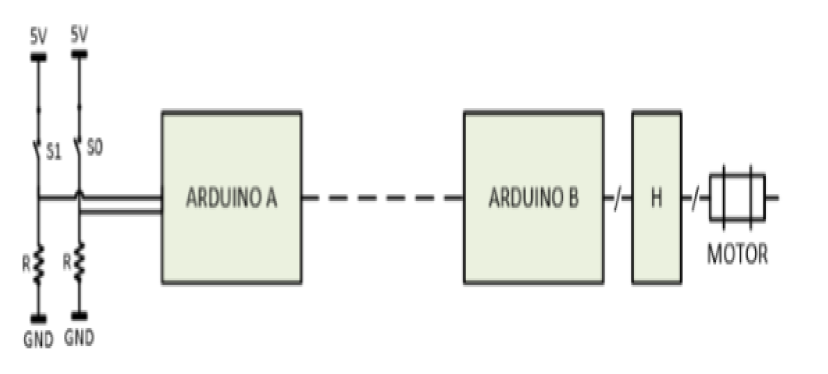
\includegraphics[width=0.45\textwidth]{Prácticas/Práctica3/I2C.jpeg}
\caption{Diagrama de conexión Arduino A y Arduino B}
\label{fig}
\end{figure}
    
    \par Es muy importante mencionar que existe el rol de maestro y esclavo y se define al Arduino A como el maestro y al Arduino B como el esclavo. Como se menciona anteriormente utilizamos el protocolo I2C en puertos establecidos del Arduino Mega para poder habilitar el canal de comunicación entre arduinos y de esta manera enviar la comunicación de los botones para poder manipular el motor basandonos en la siguiente tabla de acciones:
    \\

    \begin{center}
    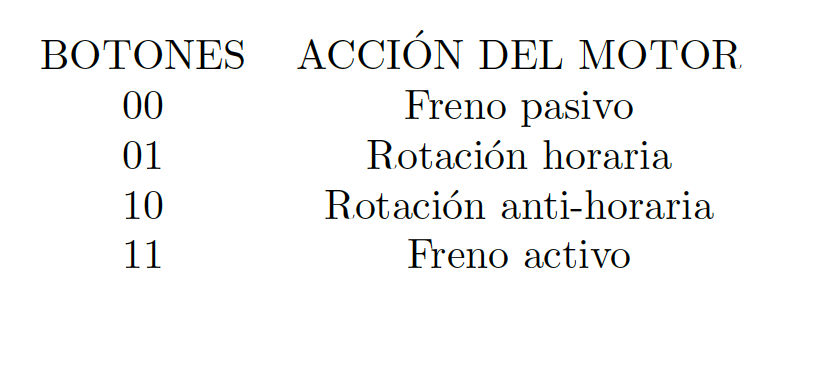
\includegraphics[width=0.28\textwidth]{Prácticas/Práctica3/accionesmotor.jpeg}
    \caption{Diagrama Acciones}
    \label{fig}
    \end{center}\\
    
    \par En una protoboard configuramos 2 botones  para poder manipular y configurar el maestro y el esclaavo. De igual manera se cableo el puente H que va conectado al motor. A continuación se muestra un diagrama del cableado:\\\\
    
    \begin{center}
    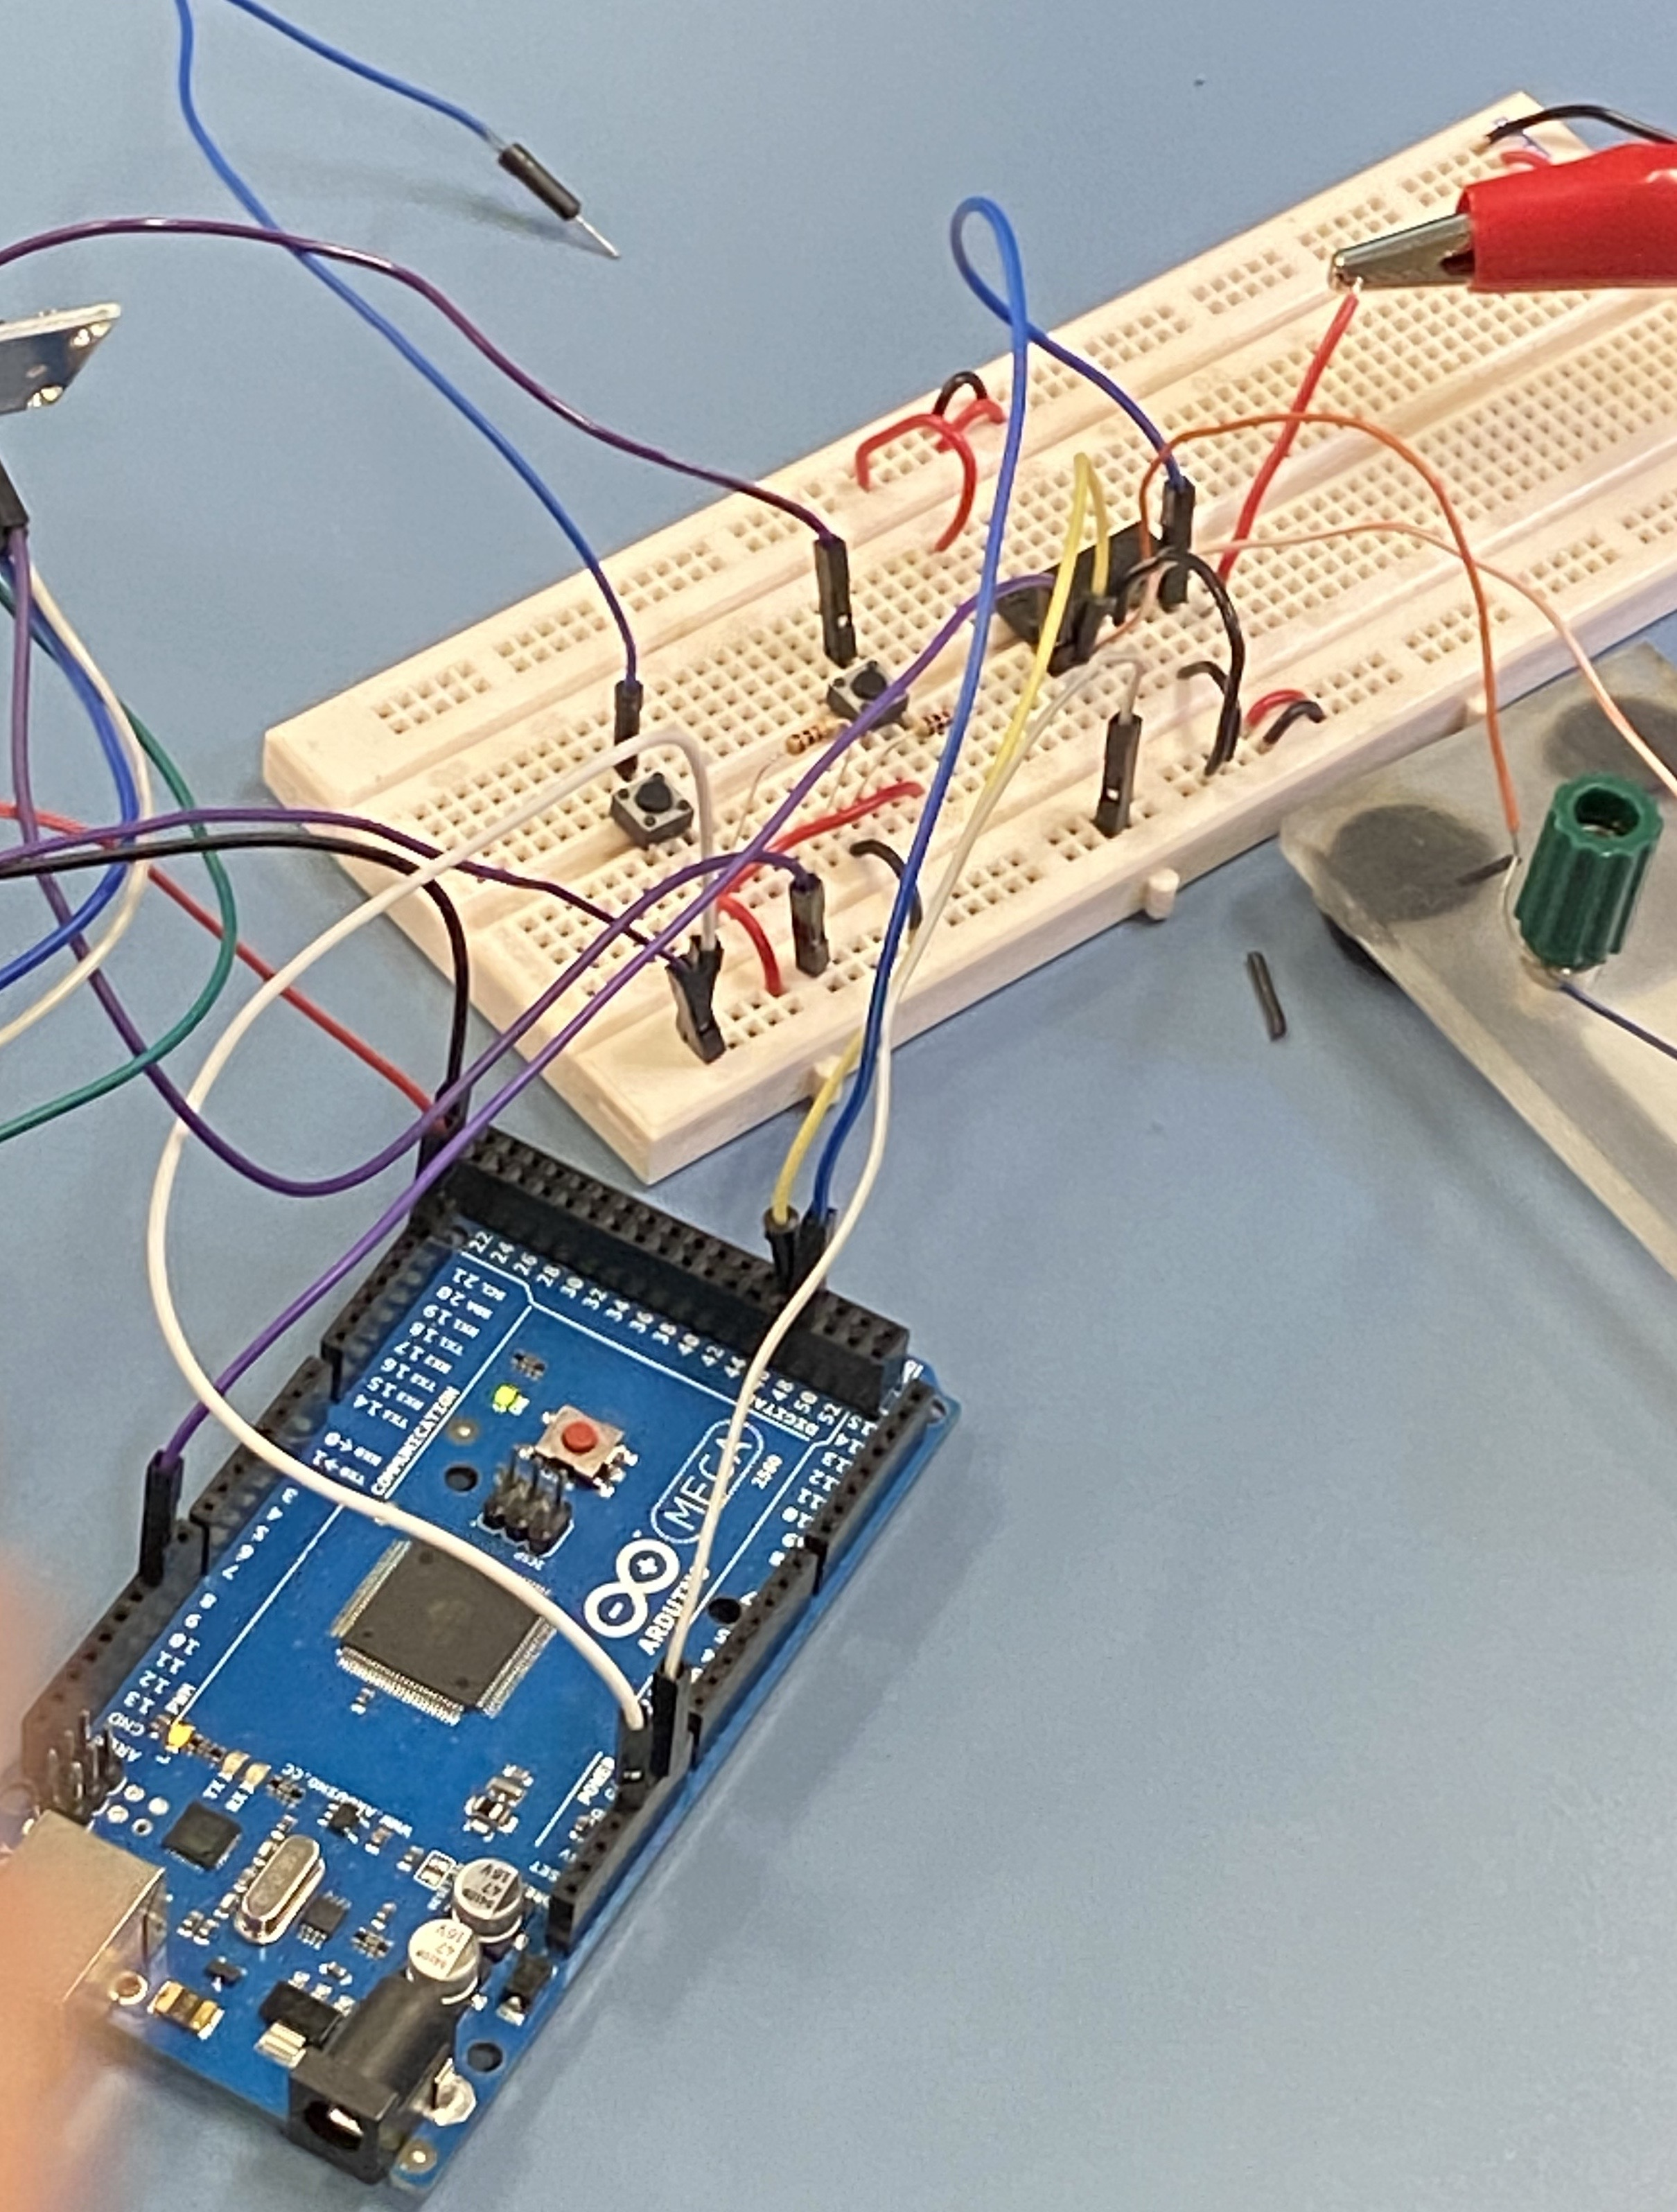
\includegraphics[width=0.30\textwidth]{Prácticas/Práctica3/practica3cabl.jpeg}\\
    \caption{Cableado}
    \label{fig}
    \end{center}  \\
    
    
    \item Acelerometro\\
    \par En esta sección vamos a aprender a utilizar un acelerometro y a integrarlo al circuito que ya tenemos armado.
    \par 
    \par El objetivo inicial es hacer que el acelerómetro recibira la posición angular en la que se encuentra  y transmitirla al Arduinno para poder ver los resultdos en el monitor serial.  El segundo punto va a ser implementar un acelerometro con el circuito del motor creado previamente.\\
    La conexión fue sencilla, se requiere utilizar los puertos GND y 5V,a continuación se conecta el pin SDA y SCL con los pines correspondientes del sensor.\\


    \item Comunicación inalámbrica\\
    
    \par En esta sección vamos a aprender a realizar la comunicación entre antenas de XBEE por medio del software XCTU. El objetivo es poder realizar comunicación inalámbrica entre los dos Arduinos (A,B). Al realizar la comunicación entre los dos modulos de igual manera debemos especificar un esclavo y un master y por medio del software definir cada antena, la segunda sección de esta practica consiste en integrar el circuito de la sección pasada pero por medio de comunicación inalámbrica. 
\end{enumerate}

\section{Resultados}\\\\

\par La práctica fue mucho de nuestro agrado por que nos permitió juntarnos con otros equipos y tener distintos puntos de vista y en conjunto encontrar los siguientes resultados.\\

\begin{itemize}
    \item En la primera parte tuvimos la oportunidad de conocer el protocolo i2c. Fue muy agradable armar el circuito y ver como el motor funcionaba con el tacto de los botones. El puente H se realizó con un circuito integrado para el funcionamiento del motor. La comunicación entre Arduinos fue satisfactoria, no se realizó el punto f ya que el protocolo ya no es utilizado mucho en la actualidad.\\
    \item La segunda parte de esta práctica fue un poco complicado entender la lógica del acelerometro y como integrar este a lo ya armado sin conocimientos previos de las librerias y de manejo.
    Se logra obtener los datos recibidos de la posición del acelerometro y ver como se comporta en la consola. Se anexa código en repositorio. Se logró observar la velocidad cambiante  dependiendo de la posición angular del acelerómetro mediante la conexión I2C.\\ Después de realizar varias pruebas poniendo prints y simular un debugeo y entender las librerias en el codigo pudimos integrar el acelerometro al circuito de la sección pasada. Al momento de mover el acelerometro se va determinado como se va a comportar el motor lo cual fue bastante interesante de observar. A continuación mostramos el circuito implementado en el circuito que maneja el motor.\\
    
    \begin{center}
    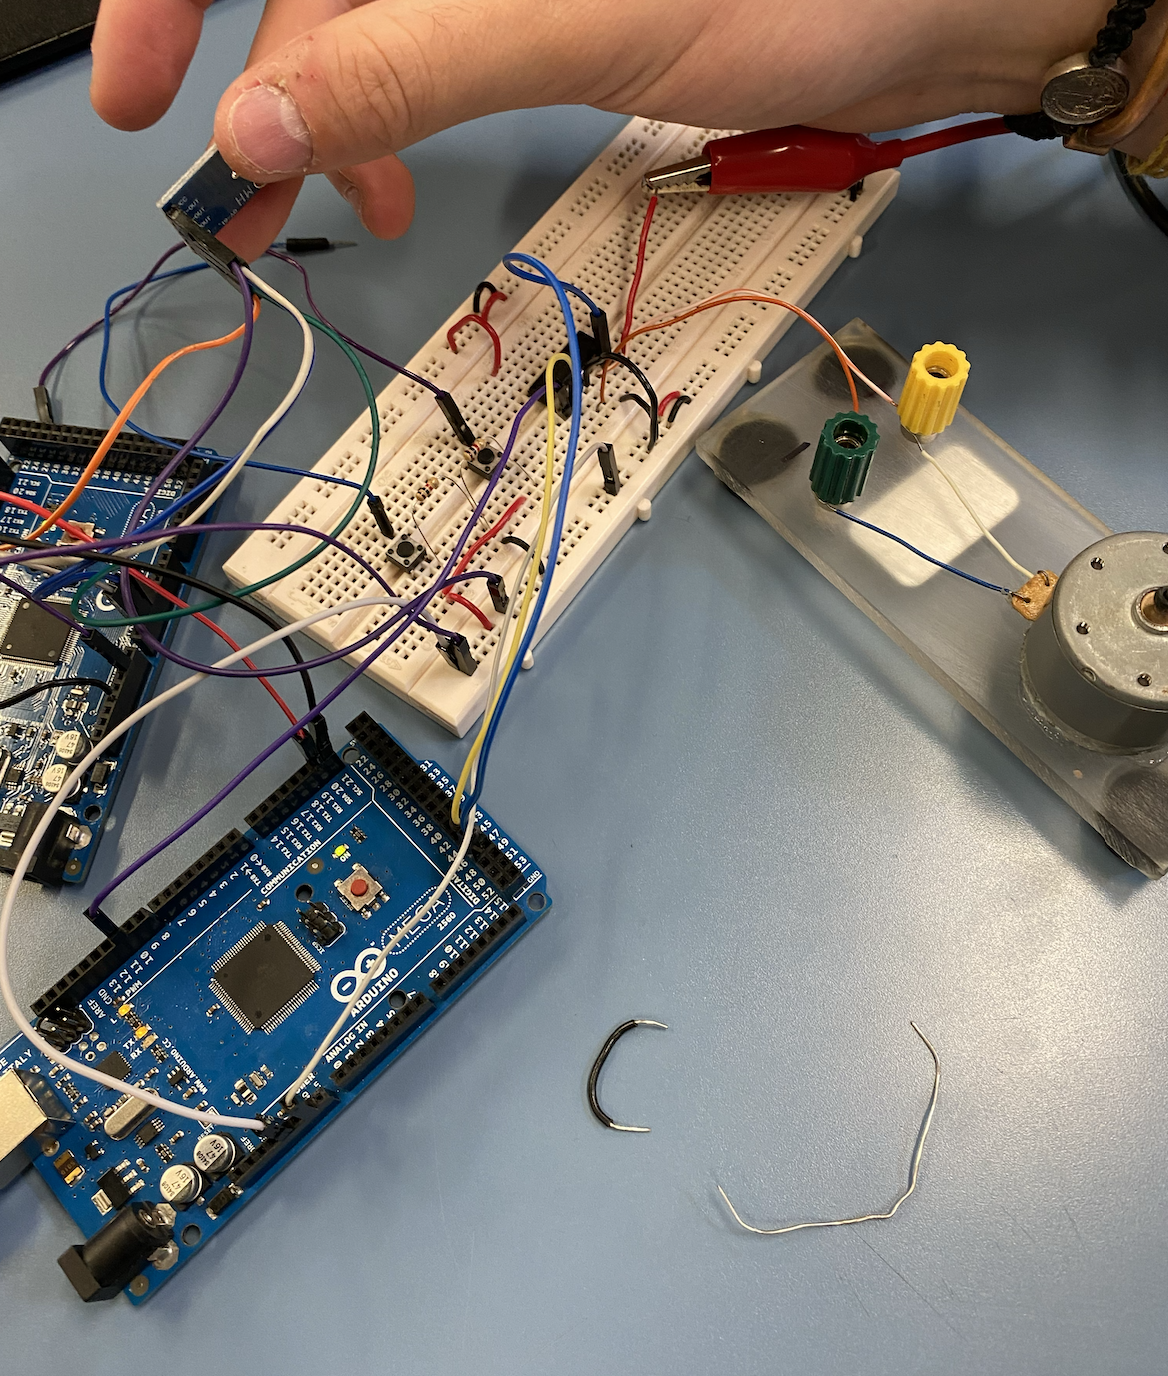
\includegraphics[width=0.35\textwidth]{Prácticas/Práctica3/prac3result.png}
    \caption{Implementación Acelerometro}
    \label{fig}
    \end{center}\\

    \item En la última parte de la práctica tuvimos que familiarizarnos con el software y el hardware de las antenas a comunicar entre Arduinos. Se utilizó la plataforma XCTU en donde se configuran el receptor y el transmisor. En esta sección tuvimos que determinar y configurar las antenas previamente antes de realizar cualquier operación sobre ellas. El profesor nos comentó que en algunas ocasiones las antenas tiene guardado información y tienen memoria por lo que al incluirlas en el software hay que borrar todo el contenido configurarlo correctamente antes de integrarlo a cualquier proyecto.\\
    
    \begin{center}
    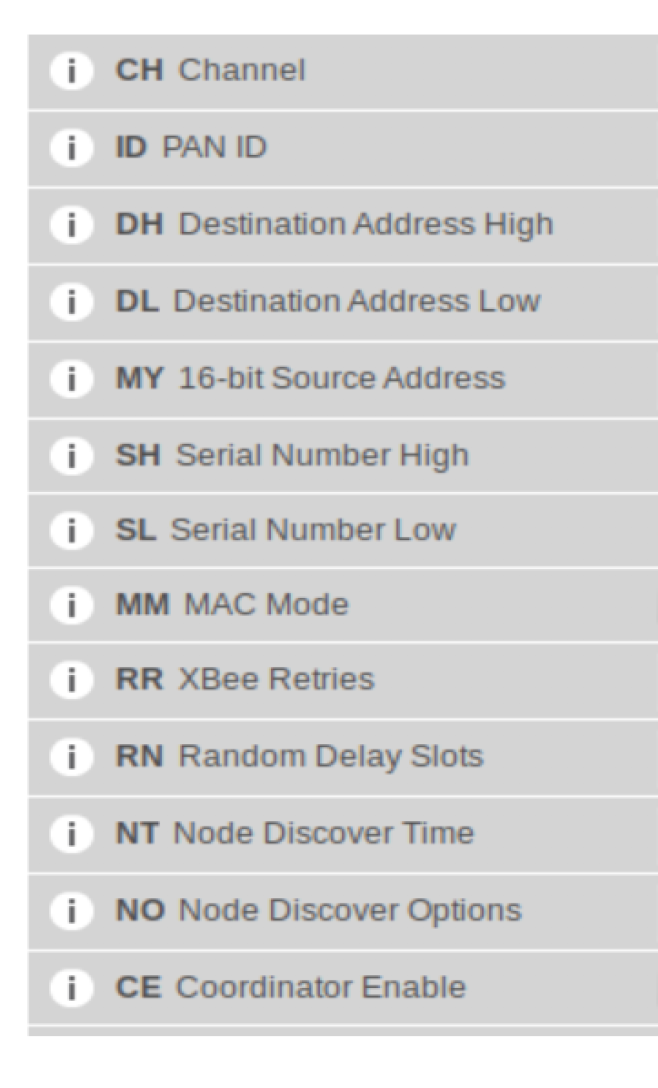
\includegraphics[width=0.35\textwidth]{Prácticas/Práctica3/xbee.jpeg}\\
    \caption{Parametros XCTU}
    \label{fig}
    \end{center}\\\\
    
    El profesor nos menciona que esto es algo común y hay que realizar muchas pruebas pero finalmente pudimos ver las antenas en el software . Otro detalle sobresaliente y que nos costó problemas en la práctica fue configurar estas antenas ya que en ocasiones funcionaba y en otras no. Finalmente logramos que la conexión entre antenas fuera correcto pero ya nos dio tiempo y contamos con muchos problemas para integrarlo al circuito previo. 

\end{itemize}


\section{Conclusiones}

\par Esta práctica nos sirvió mucho para entender diferentes protocolos de comunicación. El tema nos hizo comprender lo importante que es entender de donde provienen y la historia sobre veteranos protocolos de comunicación que incluso algunos estan todavía en uso en la actualidad. Tuvimos unas complicaciones con base en el material ya que no contamos con suficienntes acelerometros y esto nos comió tiempo importante. Consideramos que la interacción entre equipos fue bastante importante y crucial en esta práctica ya que pudimos decifrar entre todos las libreriasa y lenguajes de cada protocolo. Fue maravilloso ver como las comunincaciones son una parte importante en nuestra sociedad y verlo a esta escala fue bastante importante. 




\begin{thebibliography}{00}
\begin{itemize}
\item https://www.luisllamas.es/arduino-i2c/
\item https://www.digi.com/resources/documentation/digidocs/PDFs/90001458-13.pdf
\item https://programarfacil.com/blog/arduino-blog/conectar-dos-arduinos-i2c/
\item XBee.cl - Comunicaci´on Inal´ambrica para Tus Proyectos. 2020.
¿Qu´e Es Xbee? Xbee.Cl - Comunicaci´on Inal´ambrica Para Tus
Proyectos. [online] Available at: ¡https://xbee.cl/que-es-xbee/¿ [Accessed
13 March 2020].

\item Matic, A., Osmani, V. and Mayora, O., 2012.
Speech Activity Detection Using Accelerometer.
[online] Venetosmani.com. Available at:
¡https://venetosmani.com/publications/SpeechActivityDetectionUsingAccelerometerIEEEEMBC2012:pdf >

\item NationalInstruments:[online]Availableat :< https :
==knowledge:ni:com=KnowledgeArticleDetails?id =
kA00Z0000019MgLSAU > [Accessed13March2020]:
 Irazabal, J. and Blozis, S., 2003. AN10216-01 I 2 C MANUAL.
[online] Nxp.com. Available at: ¡https://www.nxp.com/docs/en/applicationnote/
AN10216.pdf¿ [Accessed 13 March 2020].

\end{itemize}

\end{thebibliography}

\end{document}
